% !TeX root = ../../../book.tex
\subsection{多米诺与密铺} \label{sec:section2.4.1}

这个示例比前两个稍显复杂。我们最终仍将证明某个数值公式,但问题本身比单纯操纵代数表达式更直观。此外,在开始阶段我们会注意到一个有趣的现象:必须先解决几个``小案例'',才能推广方法。这将是我们首次探讨如何调整归纳技术以适应其他情况。

我们要回答的问题可以表述如下:

\begin{quote}
    给定一个由 $2 \times n$ 个方格组成的棋盘,有多少种不同的方式能用多米诺骨牌完全覆盖(密铺)该棋盘?覆盖时每个方格必须被有且仅有一块多米诺骨牌覆盖。
\end{quote}
例如,以下是正确的密铺:

\begin{center}
    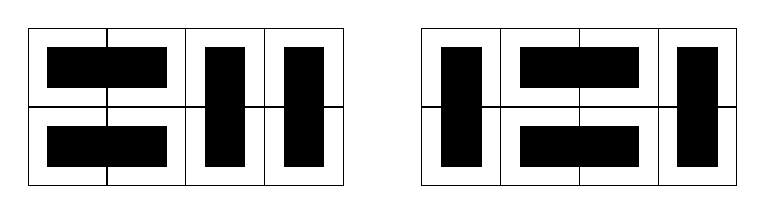
\begin{tikzpicture}[x=1.0cm, y=1.0cm]
        \foreach \y in {0,1} {
            \foreach \x in {0,...,3} {
                \draw (0+\x ,0+\y) rectangle ++ (1,1);
            }
        }

        \draw[fill, black] (0.25 ,0.25) rectangle ++ (1.5,0.5);
        \draw[fill, black] (0.25 ,1.25) rectangle ++ (1.5,0.5);
        \draw[fill, black] (2.25 ,0.25) rectangle ++ (0.5,1.5);
        \draw[fill, black] (3.25 ,0.25) rectangle ++ (0.5,1.5);

        \foreach \y in {0,1} {
            \foreach \x in {0,...,3} {
                \draw (5+\x ,0+\y) rectangle ++ (1,1);
            }
        }

        \draw[fill, black] (5+1.25 ,0.25) rectangle ++ (1.5,0.5);
        \draw[fill, black] (5+1.25 ,1.25) rectangle ++ (1.5,0.5);
        \draw[fill, black] (5+0.25 ,0.25) rectangle ++ (0.5,1.5);
        \draw[fill, black] (5+3.25 ,0.25) rectangle ++ (0.5,1.5);
    \end{tikzpicture}
\end{center}
而以下\emph{不}是正确的密铺:

\begin{center}
    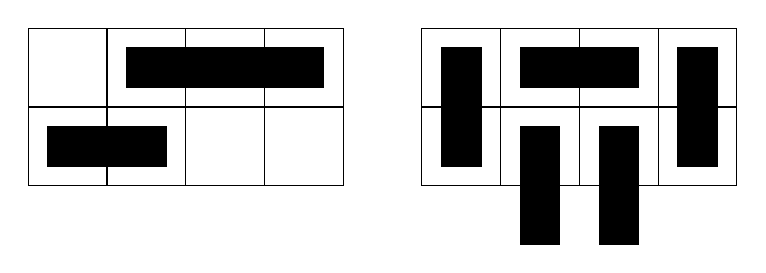
\begin{tikzpicture}[x=1.0cm, y=1.0cm]
        \foreach \y in {0,1} {
            \foreach \x in {0,...,3} {
                \draw (0+\x ,0+\y) rectangle ++ (1,1);
            }
        }

        \draw[fill, black] (0.25 ,0.25) rectangle ++ (1.5,0.5);
        \draw[fill, black] (1.25 ,1.25) rectangle ++ (1.5,0.5);
        \draw[fill, black] (2.25 ,1.25) rectangle ++ (1.5,0.5);

        \foreach \y in {0,1} {
            \foreach \x in {0,...,3} {
                \draw (5+\x ,0+\y) rectangle ++ (1,1);
            }
        }

        \draw[fill, black] (5+1.25 ,1.25) rectangle ++ (1.5,0.5);
        \draw[fill, black] (5+1.25 ,-0.75) rectangle ++ (0.5,1.5);
        \draw[fill, black] (5+2.25 ,-0.75) rectangle ++ (0.5,1.5);
        \draw[fill, black] (5+0.25 ,0.25) rectangle ++ (0.5,1.5);
        \draw[fill, black] (5+3.25 ,0.25) rectangle ++ (0.5,1.5);
    \end{tikzpicture}
\end{center}

与之前一样,先观察前几种情形($n = 1, 2, 3$ 等),尝试寻找规律。在继续阅读之前,建议先自行思考!

当 $n = 1$ 时,棋盘形状恰好与一块多米诺骨牌相同,因此仅有一种密铺方式。用 $T(n)$ 表示 $2 \times n$ 棋盘的密铺数,故 $T(1) = 1$。

\begin{center}
    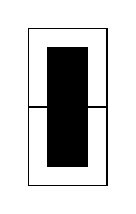
\begin{tikzpicture}[x=1.0cm, y=1.0cm]
        \draw (0,0) rectangle ++ (1,1);
        \draw (0,1) rectangle ++ (1,1);
        \draw[fill, black] (0.25 ,0.25) rectangle ++ (0.5,1.5);
    \end{tikzpicture}
\end{center}

当 $n = 2$ 时,$2 \times 2$ 棋盘有两种不同的密铺方式,此时棋盘的方向很重要,因此 $T(2) = 2$。

\begin{center}
    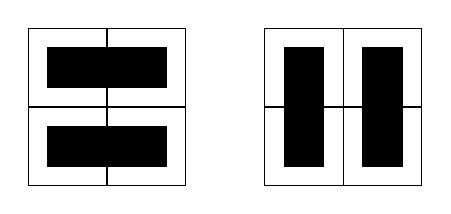
\begin{tikzpicture}[x=1.0cm, y=1.0cm]
        \foreach \y in {0,1} {
            \foreach \x in {0,1} {
                \draw (0+\x ,0+\y) rectangle ++ (1,1);
            }
        }

        \draw[fill, black] (0.25 ,0.25) rectangle ++ (1.5,0.5);
        \draw[fill, black] (0.25 ,1.25) rectangle ++ (1.5,0.5);

        \foreach \y in {0,1} {
            \foreach \x in {0,1} {
                \draw (3+\x ,0+\y) rectangle ++ (1,1);
            }
        }

        \draw[fill, black] (3+0.25 ,0.25) rectangle ++ (0.5,1.5);
        \draw[fill, black] (3+1.25 ,0.25) rectangle ++ (0.5,1.5);
    \end{tikzpicture}
\end{center}

当 $n = 3$ 时,通过枚举可得 $T(3) = 3$。

\begin{center}
    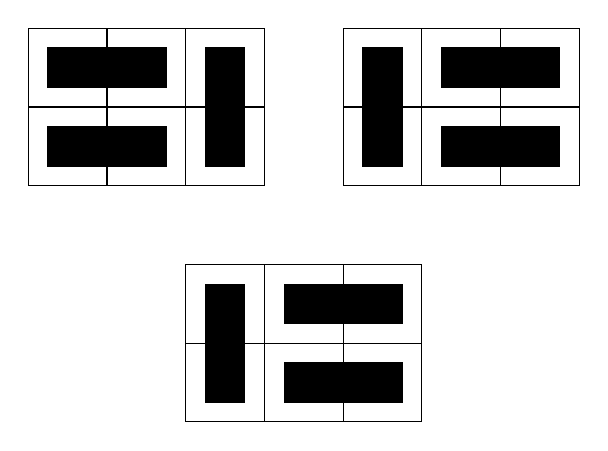
\begin{tikzpicture}[x=1.0cm, y=1.0cm]
        \foreach \y in {0,1} {
            \foreach \x in {0,1,2} {
                \draw (0+\x ,0+\y) rectangle ++ (1,1);
            }
        }

        \draw[fill, black] (0.25 ,0.25) rectangle ++ (1.5,0.5);
        \draw[fill, black] (0.25 ,1.25) rectangle ++ (1.5,0.5);
        \draw[fill, black] (2.25 ,0.25) rectangle ++ (0.5,1.5);

        \foreach \y in {0,1} {
            \foreach \x in {0,1,2} {
                \draw (4+\x ,0+\y) rectangle ++ (1,1);
            }
        }

        \draw[fill, black] (4+1.25 ,0.25) rectangle ++ (1.5,0.5);
        \draw[fill, black] (4+1.25 ,1.25) rectangle ++ (1.5,0.5);
        \draw[fill, black] (4+0.25 ,0.25) rectangle ++ (0.5,1.5);

        \foreach \y in {0,1} {
            \foreach \x in {0,1,2} {
                \draw (2+\x ,-3+\y) rectangle ++ (1,1);
            }
        }

        \draw[fill, black] (2+1.25 ,-3+0.25) rectangle ++ (1.5,0.5);
        \draw[fill, black] (2+1.25 ,-3+1.25) rectangle ++ (1.5,0.5);
        \draw[fill, black] (2+0.25 ,-3+0.25) rectangle ++ (0.5,1.5);
    \end{tikzpicture}
\end{center}

再看 $n=4$ 的情形,可验证 $T(4)=5$。

\begin{center}
    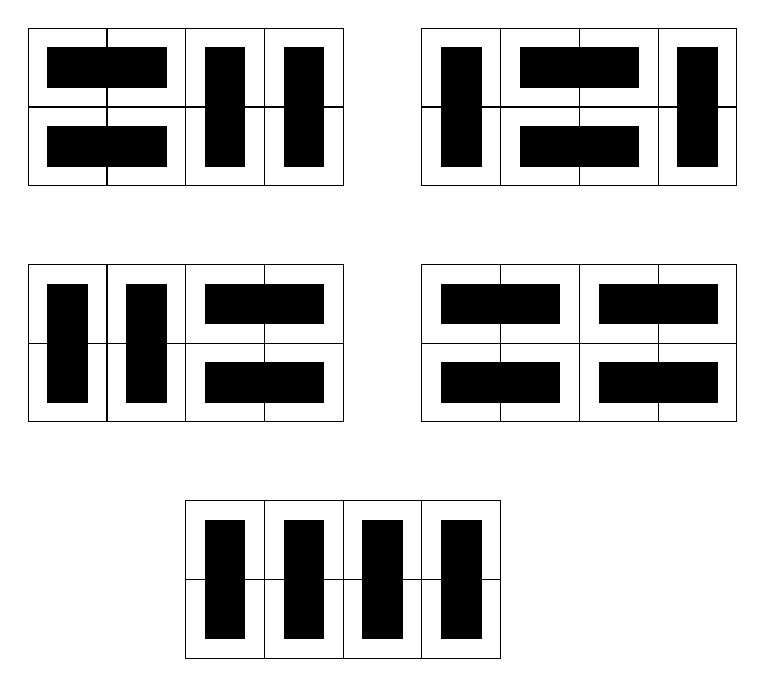
\begin{tikzpicture}[x=1.0cm, y=1.0cm]
        \foreach \y in {0,1} {
            \foreach \x in {0,...,3} {
                \draw (0+\x ,0+\y) rectangle ++ (1,1);
            }
        }

        \draw[fill, black] (0.25 ,0.25) rectangle ++ (1.5,0.5);
        \draw[fill, black] (0.25 ,1.25) rectangle ++ (1.5,0.5);
        \draw[fill, black] (2.25 ,0.25) rectangle ++ (0.5,1.5);
        \draw[fill, black] (3.25 ,0.25) rectangle ++ (0.5,1.5);

        \foreach \y in {0,1} {
            \foreach \x in {0,...,3} {
                \draw (5+\x ,0+\y) rectangle ++ (1,1);
            }
        }

        \draw[fill, black] (5+1.25 ,0.25) rectangle ++ (1.5,0.5);
        \draw[fill, black] (5+1.25 ,1.25) rectangle ++ (1.5,0.5);
        \draw[fill, black] (5+0.25 ,0.25) rectangle ++ (0.5,1.5);
        \draw[fill, black] (5+3.25 ,0.25) rectangle ++ (0.5,1.5);

        \foreach \y in {0,1} {
            \foreach \x in {0,...,3} {
                \draw (0+\x ,-3+\y) rectangle ++ (1,1);
            }
        }

        \draw[fill, black] (2.25 ,-3+0.25) rectangle ++ (1.5,0.5);
        \draw[fill, black] (2.25 ,-3+1.25) rectangle ++ (1.5,0.5);
        \draw[fill, black] (0.25 ,-3+0.25) rectangle ++ (0.5,1.5);
        \draw[fill, black] (1.25 ,-3+0.25) rectangle ++ (0.5,1.5);

        \foreach \y in {0,1} {
            \foreach \x in {0,...,3} {
                \draw (5+\x ,-3+\y) rectangle ++ (1,1);
            }
        }

        \draw[fill, black] (5+2.25 ,-3+0.25) rectangle ++ (1.5,0.5);
        \draw[fill, black] (5+2.25 ,-3+1.25) rectangle ++ (1.5,0.5);
        \draw[fill, black] (5+0.25 ,-3+0.25) rectangle ++ (1.5,0.5);
        \draw[fill, black] (5+0.25 ,-3+1.25) rectangle ++ (1.5,0.5);

        \foreach \y in {0,1} {
            \foreach \x in {0,...,3} {
                \draw (2+\x ,-6+\y) rectangle ++ (1,1);
            }
        }

        \draw[fill, black] (2+0.25 ,-6+0.25) rectangle ++ (0.5,1.5);
        \draw[fill, black] (2+1.25 ,-6+0.25) rectangle ++ (0.5,1.5);
        \draw[fill, black] (2+2.25 ,-6+0.25) rectangle ++ (0.5,1.5);
        \draw[fill, black] (2+3.25 ,-6+0.25) rectangle ++ (0.5,1.5);
    \end{tikzpicture}
\end{center}

现在能否寻找规律?手工计算更大棋盘的密铺数过于繁琐。尝试利用 $T(1) = 1$ 推导 $T(2)$……但无法实现,因为两情形本质不同:多米诺骨牌尺寸为 $2 \times 1$,仅添加一行不足以建立联系。

那么考虑 $n = 3$。能否利用 $T(2) = 2$?答案是肯定的!已知 $2 \times 2$ 棋盘有两种密铺,可直接将其扩展:在每种密铺右侧\emph{添加竖直多米诺骨牌},得到两种 $2 \times 3$ 密铺。但实际上 $T(3) = 3$,第三种密铺从何而来?观察发现,第三种密铺右侧为两块水平放置的多米诺骨牌。若移去这两块骨牌,剩余部分即 $n=1$ 的情形。换言之,第三种密铺是通过在 $2 \times 1$ 棋盘右侧\emph{添加两块水平骨牌}构成的。综上,$2 \times 3$ 棋盘的所有密铺均可由较小尺寸($2 \times 2$ 和 $2 \times 1$)导出:

\begin{center}
    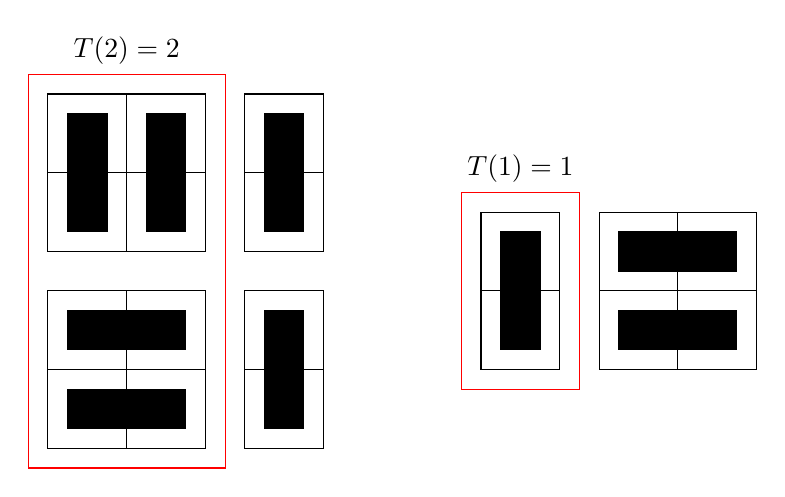
\begin{tikzpicture}[x=1.0cm, y=1.0cm]
        \foreach \g in {0, 2.5} {
            \foreach \y in {0,1} {
                \foreach \x in {0,1} {
                    \draw (0+\x ,0+\y+\g) rectangle ++ (1,1);
                }
            }
            \draw (2.5,0+\g) rectangle ++ (1,1);
            \draw (2.5,1+\g) rectangle ++ (1,1);
            \draw[fill, black] (2.75 ,0.25+\g) rectangle ++ (0.5,1.5);
        }

        \draw[fill, black] (0.25 ,0.25) rectangle ++ (1.5,0.5);
        \draw[fill, black] (0.25 ,1.25) rectangle ++ (1.5,0.5);

        \draw[fill, black] (0.25 ,2.5+0.25) rectangle ++ (0.5,1.5);
        \draw[fill, black] (1.25 ,2.5+0.25) rectangle ++ (0.5,1.5);

        \draw[red] (-0.25, -0.25) rectangle ++(2.5, 5);
        \path (-0.25,4.75) --  (2.25,4.75) node[midway,above,black] {$T(2)=2$};

        \draw (5.5,1) rectangle ++ (1,1);
        \draw (5.5,2) rectangle ++ (1,1);
        \draw[fill, black] (5.75 ,1.25) rectangle ++ (0.5,1.5);
        \draw[red] (5.25, 0.75) rectangle ++(1.5, 2.5);
        \path (5.25,3.25) --  (6.75,3.25) node[midway,above,black] {$T(1)=1$};

        \foreach \y in {0,1} {
            \foreach \x in {0,1} {
                \draw (7+\x ,1+\y) rectangle ++ (1,1);
            }
        }
        \draw[fill, black] (7.25 ,1.25) rectangle ++ (1.5,0.5);
        \draw[fill, black] (7.25 ,2.25) rectangle ++ (1.5,0.5);

    \end{tikzpicture}
\end{center}
\[T(3) = 3 = 2 + 1 = T(2) + T(1)\]

规律初现!再验证 $n = 4$:向 $T(3)$ 的每种密铺添加竖直骨牌,或向 $T(2)$ 的每种密铺添加两块水平骨牌,即可得到 $T(4)$ 的\emph{所有}密铺:

\begin{center}
    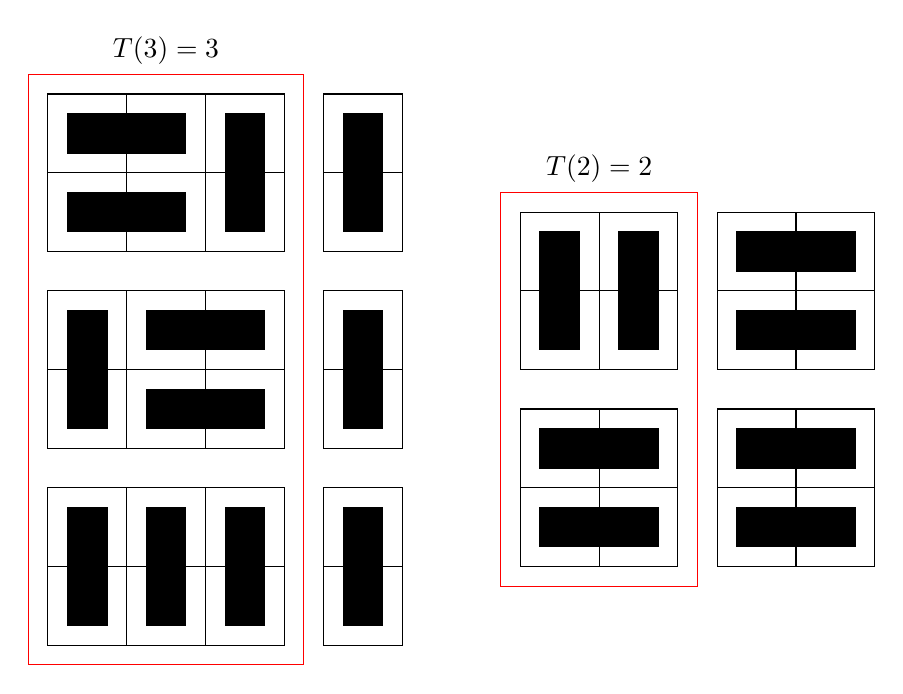
\begin{tikzpicture}[x=1.0cm, y=1.0cm]
        \foreach \g in {0, 2.5, 5} {
            \foreach \y in {0,1} {
                \foreach \x in {0,1,2} {
                    \draw (0+\x ,0+\y+\g) rectangle ++ (1,1);
                }
            }

            \draw (3.5,\g+0) rectangle ++ (1,1);
            \draw (3.5,\g+1) rectangle ++ (1,1);
            \draw[fill, black] (3.75 ,\g+0.25) rectangle ++ (0.5,1.5);
        }
        \draw[fill, black] (0.25 ,0.25) rectangle ++ (0.5,1.5);
        \draw[fill, black] (1.25 ,0.25) rectangle ++ (0.5,1.5);
        \draw[fill, black] (2.25 ,0.25) rectangle ++ (0.5,1.5);

        \draw[fill, black] (0.25 ,2.75) rectangle ++ (0.5,1.5);
        \draw[fill, black] (1.25 ,2.75) rectangle ++ (1.5,0.5);
        \draw[fill, black] (1.25 ,3.75) rectangle ++ (1.5,0.5);

        \draw[fill, black] (2.25 ,5.25) rectangle ++ (0.5,1.5);
        \draw[fill, black] (0.25 ,5.25) rectangle ++ (1.5,0.5);
        \draw[fill, black] (0.25 ,6.25) rectangle ++ (1.5,0.5);

        \draw[red] (-0.25, -0.25) rectangle ++(3.5, 7.5);
        \path (-0.25,7.25) --  (3.25,7.25) node[midway,above,black] {$T(3)=3$};


        \foreach \g in {0, 2.5} {
            \foreach \y in {0,1} {
                \foreach \x in {0,1} {
                    \draw (6+\x ,1+\y+\g) rectangle ++ (1,1);
                }
            }
            \foreach \y in {0,1} {
                \foreach \x in {0,1} {
                    \draw (8.5+\x ,1+\y+\g) rectangle ++ (1,1);
                }
                \draw[fill, black] (8.75 ,1.25+\g+\y) rectangle ++ (1.5,0.5);
            }
           
        }

        \draw[fill, black] (6.25 ,1.25) rectangle ++ (1.5,0.5);
        \draw[fill, black] (6.25 ,2.25) rectangle ++ (1.5,0.5);

        \draw[fill, black] (6.25 ,3.5+0.25) rectangle ++ (0.5,1.5);
        \draw[fill, black] (7.25 ,3.5+0.25) rectangle ++ (0.5,1.5);

        \draw[red] (5.75, 0.75) rectangle ++(2.5, 5);
        \path (5.75,5.75) --  (8.25,5.75) node[midway,above,black] {$T(2)=2$};
        
    \end{tikzpicture}
\end{center}
\[T(4) = 5 = 3 + 2 = T(3) + T(2)\]

需要注意的是,此方式不会产生重复密铺。(仔细思考为何能保证唯一性?)由此可直接推出 $T(4) = T(3) + T(2)$。

此外,上述论证具有普适性。对于任意 $n$,观察棋盘最右侧:若为竖直骨牌,则密铺源于 $2 \times (n - 1)$ 棋盘;若为水平骨牌对,则源于 $2 \times (n-2)$ 棋盘。因此对所有满足条件的 $n$ 有:
\[T(n) = T(n - 1) + T(n - 2)\]
哪些 $n$ 值适用?请记住,我们必须单独分析 $T(1)$ 和 $T(2)$;因此上述公式不适用于 $n=1$ 和 $n=2$,我们必须添加限制条件 $n \ge 3$ 才能使上面公式成立。

据此可轻松计算任意 $n$ 对应的 $T(n)$,甚至可编程实现。但正是\emph{归纳}论证——对模式的细致观察及其成因的透彻分析——使我们得出最终结论。本例中,$T(n)$ 的值依赖于前两项 $T(n-1)$ 和 $T(n-2)$,这在前文示例中\emph{未曾}出现,这暗示了更深层的机制。是否察觉此前的归纳定义与多米诺骨牌类比在此失效?如何修正类比以解释此情况?思考一下这些问题,然后再继续阅读。我们将在下一个示例之后深入讨论它们。

顺便一提,你是否注意到此数列的特别之处?你还知道其他类似的数列吗?思考一下吧……
